
\subsection{Соединения олова и кремния, способы получения, химическое поведение, электронное и геометрическое строение молекул}

\subsubsection*{Si и Sn}

\textbf{Получение}

1) Si - в лаборатории

$$SiO_2 + Mg \rightarrow Si + MgO$$
$$SiO_2 + Al \rightarrow Si + Al_2O_3$$

2) Si в промышленности

$$SiO_2 + C \rightarrow Si +  CO$$
$$SiCl_4 + H_2 \xrightarrow{1200^{\circ}} Si + HCl$$
$$SiCl_4 + Zn \rightarrow Si + ZnCl_2$$
$$SiH_4 \rightarrow Si + H_2$$

3) Sn - из минерала касситерита

$$SnO_2 + C \rightarrow Sn + CO_2$$

\textbf{Химические свойства}

Si

1) С $Hal_2$

$$Si + 2F_2 \rightarrow SiF_4$$
$$Si + X_2 \rightarrow SiX_4 (X = Cl, Br, I)$$

2) С $O_2$

$$Si + O_2 \xrightarrow{600^{\circ}} SiO_2$$

3) С другими неметаллами

$$Si + C \xrightarrow{1000^{\circ}} SiC$$
$$Si + N_2 \rightarrow Si_3N_4$$
$$Si + S \xrightarrow{250-600^{\circ}} SiS_2$$
$$Si + B \rightarrow SiB_{3x} (x = 1,2,4)$$

4) Метод Рохова-Петноуда

$$Si + CH_3Cl \xrightarrow[250-300^{\circ}]{Cu} \frac{(C_2H_5)_2SiCl_2}{70-90^{\circ}} + HSiCl_3 + disilan + ...$$

Много побочных соединений, которые потом подвергаются ректификации

5) С металлами

$$Si + Me \rightarrow Me_nSi_m$$

6) С $OH^-$

$$Si + NaOH + H_2O \rightarrow Na_2SiO_3 + H_2 \uparrow$$

7) С галогенводородами

$$Si + HX \rightarrow SiX_4 + H_2$$

(X = $F$(н.у) , $Cl (300^{\circ}), Br(500^{\circ}$))

8) Устойчив к действию кислот, кроме реакции:

$$Si + HNO_{3(konc)} + HF_{(konc)} \xrightarrow[-NO-H_2O]\ H_2[SiF_6]$$

$Sn$

1) При $t^{\circ}$ с $Hal_2, O_2, S$

$$Sn + Cl_2 \rightarrow SnCl_4$$
$$Sn+ S \rightarrow SnS (SnS_2)$$
$$Sn + O_2 \xrightarrow{200^{\circ}} SnO_2$$

2) Растворим в $HR$

$$Sn + HCl \rightarrow SnCl_2 + H_2$$

3) С кислотами и окислителями


$$Sn + HNO_{3(konc)} \rightarrow SnO_2 + NO_2 + H_2O$$

4) С $OH^-$  при $t^{\circ}$

$$Sn + KOH + H_2O \rightarrow K_2[Sn(OH)_6] + H_2$$

5) С растворами ЩМ в $NH_{3(liq)}$

$$K + Sn + en \xrightarrow{NH_{3(liq)}} [K(en)]_2Sn_5$$

Анионы Цинтля $[K(en)]_3Sn_9$

\textbf{Строение}

Si - кубическая решетка типа алмаза (ГЦК)

Модификации Sn: 

- Белое $\beta$-олово, тетрагональное, устойчиво при комнатной температуре

- Серое $\alpha$-олово, кубическая алмазная структура

Si, Sn - полупроводники


\subsubsection*{Гидриды вида $E_nH_{2n+2}$ , наиболее изучены $EH_4$}

\textbf{Получение}

$SiH_4$ - силан

$$Mg_2Si + HCl \rightarrow MgCl_2 + SiH_4$$
$$SiCl_4 + Li[AlH_4] \xrightarrow{Et_2O} SiH_4 + AlCl_3 + LiCl$$

$SnH_4$ - станнан

Аналогично $SH_4$

\textbf{Химические свойства}

1) Самовоспламенение на воздухе

$SiH_4$

$$SiH_4 + O_2 \rightarrow SiO_2 + H_2O$$

2) Разложение

$$SiH_4 \xrightarrow{500^{\circ}} Si + H_2$$

3) С $OH^-$

$$SiH_4 + NaOH + H_2O \rightarrow Na_2SiO_3 + H_2$$

4) С $Hal_2$

$$SiH_4 + Cl_2 \rightarrow SiCl_4 + HCl$$

5) Сильный окислитель

$$SiH_4 + KMnO_4 \rightarrow MnO_2\downarrow + SiO_2\downarrow + KOH + H_2O$$
$$SiH_4 + AgCl \rightarrow SiH_3Cl + HCl + Ag$$

$SnH_4$

1) Неустойчив 

$$S_nH_4 \rightarrow Sn + H_2$$

2) Самовоспламенение на воздухе

$$S_nH_4 + Hal_2 \rightarrow SnHal_4 + HHal$$

3) Сильный восстановитель

\textbf{Строение}

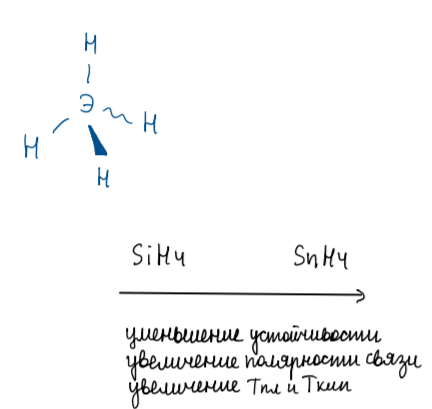
\includegraphics{images/10v1.png}

\subsubsection*{Дигалогениды}

Дигалогениды Si неустойчивы, но у Sn есть

\textbf{Получение}

1) Сопропорционирование

$$SnBr_3 + Sn \rightarrow SnBr_2$$

\textbf{Химические свойства}

1) Растворимы в воде

2) Сильные восстановители

$$SnCl_2 + H_2SO_4 + HCl \rightarrow S + H_2[SnCl_6] + H_2O$$

\textbf{Строение}

Газ - мокулярная форма,\\
Твердое - объединение в циклы, цепи, слои\\

$SnCl_2$ кристаллизуется в растворе в виде $SnCl_2\cdot 2H_2O$, причем одна кристаллическая вода не связана с Sn
 
$[SnCl_2(H_2O)](H_2O)$

В газовой фазе и в кристалле не образует соединений с кратной связью, подобно дихиоркарбену, но молекулы ассоциированы Д/А связами

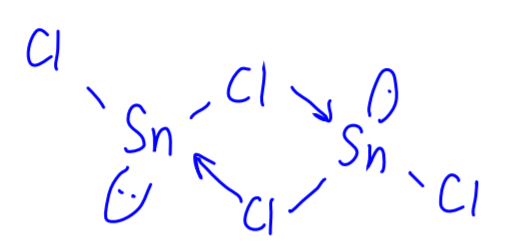
\includegraphics{images/10v2.png}

\subsubsection*{Тетрагалогениды}

Тетрагалогениды есть и у Si, и у Sn

$SiX_4$

\textbf{Получение}

$$Si (SiC) + Cl_2 \rightarrow SiCl_4$$

\textbf{Химические свойства}

1) $SiF_4$ легко присоединяет $F^-$

$$SiF_4 + KF \rightarrow K_2SiF_6$$

2) $SiX_4$ гидролизуются (x=Cl,Br,I)

$$SiX_4 + H_2O \rightarrow SiO_2\cdot nH_2O + HX$$

3) $SiF_4$ при гидролизе реагирует с HF

$$SiF_4 + H_2O \rightarrow SiO_2\cdot nH_2O HF + H_2[SiF_6]$$

$$EtMgCl + SiCl_3 \rightarrow EtSiCl_3 + Et_3SiCl + Et_2SiCl_2$$

У реакции много недостатков (мало целевого вещества, с $CH_3MgCl$ не реагирует, нужны инертная атмосфера и высокочистые реагенты)

\textbf{Строение}

Молекулы с формой правильного тетраэдра\\
\\

$SnX_4$

\textbf{Получение}

1) Прямое галогенирование

2) $SnCl_3 + HF_{bezvodn} \rightarrow SnF_4 + HCl$

\textbf{Химические свойства}

2) Легко присоединяет $X^-$ (X = F, Cl, Br, I)

$$SnCl_4 + Cl_2 \rightarrow Cl_2SnCl_6$$

2) Гидролиз при н.у. (кроме $SnF_4$)

$$SnI_4 + H_2O \rightarrow SnOI_2 + HI$$

3) $SnI_4$ - разложение

$$SnI_4 \xrightarrow{\approx 360^{\circ}} SnI_2 + I_2$$

4) $SnCl_4$ - исходное вещество для получения оловоорганики

$$SnCl_4 \xrightarrow{4RMgCl} R_4Sn \xrightarrow{nSnCl_4} R_xSnCl_{4-x } \rightarrow ...$$
Реакции нуклеофильного замещения, восстановления

\textbf{Строение}

$SnX_4 (X = Cl, Br, I)$ - аналогично $SiX_4$

$SnF_4$ состоит из полимерных цепей  с октаэдрической координацией вокруг Sn

Вниз по 14 группе E(Э-Э) падает, следовательно соединения со связью Sn-Sn легко диссоциируют с образованием радикалов

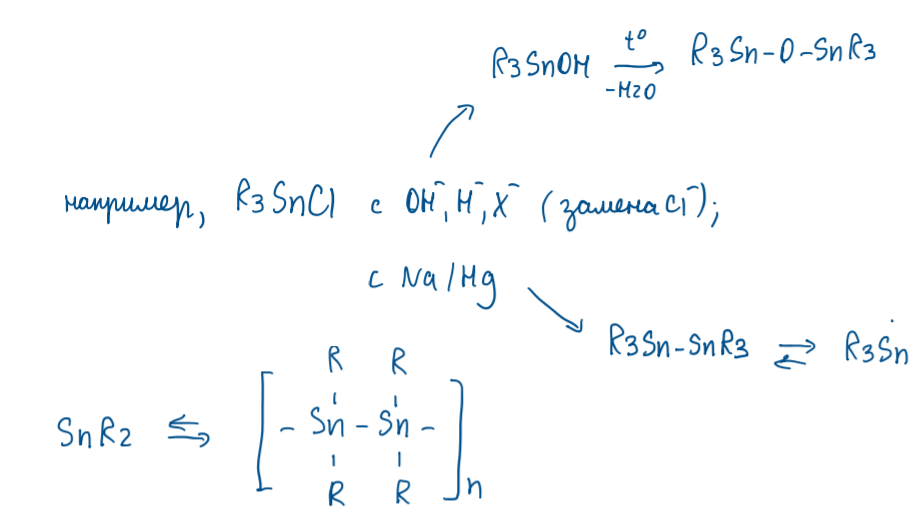
\includegraphics{images/10v3.png}

\subsubsection*{SiO и SnO}


$SiO$

\textbf{Получение}

$$SiO_2 + Si \rightarrow SiO$$

\textbf{Химические свойства}

1) Медленное разложение

$$SiO \rightarrow SiO_2 + Si$$

2) Сильный восстановитель

$$SiO + Cl_2 \rightarrow SiCl_4 + O_2$$
$$SiO + CO_2 \rightarrow SiO_2 + CO$$

\textbf{Строение}

НЭП на Si: 
\includegraphics{images/10v4.png}\\
\\
$SnO$

\textbf{Получение}

$$SnC_2O_4 \rightarrow SnO + CO + CO_2$$
$$SnCl_2 + NH_3 + H_2O \rightarrow SnO + NH_4Cl$$

\textbf{Химические свойства}

$$SnO \xrightarrow{>380^{\circ}} SnO_2 + Sn$$
$$SnO + O_2 \xrightarrow{>270^{\circ}} SnO_2$$

Амфотерный оксид $\Rightarrow$ легко с $H^+, OH^-$

\textbf{Строение}

Слоистая структура из квадратных пирамид
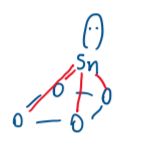
\includegraphics{images/10v5.png}

\subsubsection*{$SiO_2$ и $SnO_2$}

$SiO_2$

\textbf{Получение}

$$Si + O_2 \rightarrow SiO_2$$

Широко распространен в природе в виде песка, кварца, кремнезёма

\textbf{Химические свойства}

1)$SiO_2 + H_2O \nrightarrow$

2)С $OH^-$ при нагревании

$$SiO_2 + KOH \rightarrow K_2SiO_3 + H_2O$$

3) С основными оксидами при нагревании

4) С $CO_3^{2-}$ щм при нагревании

$$SiO_2 + K_2CO_3 \rightarrow K_2SiO_3 + CO_2$$

5) С активными металлами

$$SiO_2 + Mg \xrightarrow{izb} Mg_2Si + MgO$$
$$SiO_2 + K_2CO_3 \xrightarrow{ned} MgO + Si$$

6) С неметаллами

$$SiO_2 + H_2 \rightarrow Si + H_2O$$
$$SiO_2 + C \rightarrow SiC + CO$$
$$SiO_2 + F_2 \rightarrow SiF_4+ O_2$$

7) С $HF$

$$SiO_2 + HF \rightarrow SiF_4\uparrow + H_2O$$
$$SiO_2 + HF \rightarrow H_2[SiF_6] + H_2O$$

\textbf{Строение}

1) Кварц\\
2) Тридимит\\
3) Кристаллобалит

У всех низкотемпературных $\alpha$-формы, а выкосотемпературных $\beta$-формы

Построены из тетраэдров $SiO_4$, соед. с соседними тетраэдрами всеми атомами О в 3D-решетке

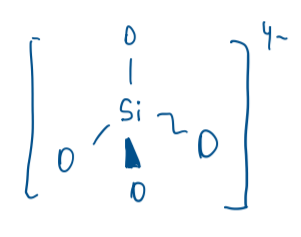
\includegraphics{images/10v6.png}\\

$SnO_2$

\textbf{Получение}

$$Sn + O_2 \xrightarrow{>220^{\circ}} SnO_2$$
$$SnO + O_2 \xrightarrow{220^{\circ}} SnO_2$$
$$SnO \xrightarrow{>380^{\circ}} SnO_2 + Sn$$
$$Sn + HNO_{3(konc)}\rightarrow SnO_2 + NO_2 + H_2O$$

\textbf{Химические свойства}

1) с Расплавами и  растворами конц. $OH^-$

$$SnO_2 + NaOH \xrightarrow{350-400^{\circ}} Na_2SnO_3 + H_2O$$
$$SnO_2 + NaOH + H_2O\xrightarrow{60-70^{\circ}} Na_2[Sn(OH)_6]$$

2) С концентрированными и разбавленными кислотами при нагревании

$$SnO_3 + HCl_{konc} \rightarrow H_2SnCl_6 + H_2O$$
$$SnO_2 + H_2SO_{4(razb)} \xrightarrow{100^{\circ}} Sn(SO_4)_2 + H_2O$$

3) Восстановление до Sn

$$SnO_2 + H_2 \xrightarrow{500-600^{\circ}} Sn + H_2O$$
$$SnO_2 + C \xrightarrow{800-900^{\circ}} Sn + CO$$

\textbf{Строение}

Диамагнитен\\
Структура типа рутила.

\subsubsection*{Кислоты Si и Sn}

$H_2SiO_3$

\textbf{Получение}

1) $SiO_3^{2-} + H^+$ (даже $H_2CO_3$)

2) $SiH_2Cl_2 + H_2O \rightarrow H_2SiO_3 + HCl + H_2$

3) Получение солей:

$$H_4SiO_4 + KOH \rightarrow K_4SiO_4 + H_2O$$
$$Si + NaOH + H_2O \rightarrow Na_2SiO_3 + H_2$$
$$SiO_2 + KOH \rightarrow K_2SiO_3 + H_2O$$
$$CaO + SiO_2 \rightarrow CaSiO_3$$

\textbf{Химические свойства}

1) С $OH^-$

$$H_4SiO_4 + KOH \rightarrow K_4SiO_4 + H_2O$$

2) Разложение 

$$H_2SiO_3 \rightarrow H_2O + SiO_2$$

3) С HF

$$H_2SiO_3 + HF \rightarrow H_2SiF_6 + H_2O + SiF_4\uparrow$$

\textbf{Строение}

Полимерные вещества - цепочки $SiO_4$ тетраэдров, связанных общими вершинами

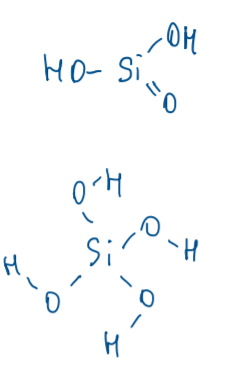
\includegraphics{images/10v7.png}

$H_2[SiF_6]$

\textbf{Получение}

$$SiF_4 + HF \rightarrow H_2SiF_6 + H_2O$$
$$SiF_4 + H_2O \rightarrow SiO_2\cdot nH_2O + HF + H_2SiF_6$$
$$SiF_4 + H_2O \rightarrow Na_2SiF_6$$

\textbf{Химические свойства}

$$H_2SiF_6 \rightarrow HF + SiF_4$$
Распадается в свободном состоянии

Сильная кислота


\textbf{Строение}

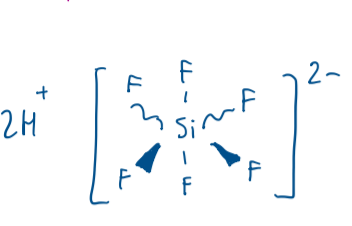
\includegraphics{images/10v8.png}

$H_2[SnCl_6]$

\textbf{Получение}

$$Sn + HNO_3 + HCl \rightarrow H_2[SnCl_6] + NO + H_2O$$
$$SnO_2 + HCl \rightarrow H_2[SnCl_6] + H_2O$$\\
$$SnCl_4 + HCl \rightarrow H_2[SnCl_6]$$

\textbf{Химические свойства}

1) С щелочами

$$H_2[SnCl_6] + NaOH_{konc} \rightarrow Na_2[Sn(OH)_6] + NaCl + H_2O$$
$$H_2[SnCl_6] + NaOH_{razb} Na_2[SnCl_6] + H_2O$$

2) C $H_2S$

$$H_2[SnCl_6] + H_2S \rightarrow SnS_2 + HCl$$

3) С Sn

$$H_2[SnCl_6] + Sn \rightarrow H[SnCl_3]$$

\textbf{Строение}

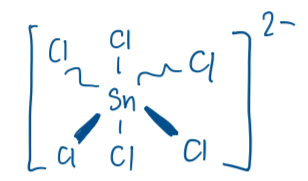
\includegraphics{images/10v9.png}